\documentclass[a4paper,titlepage]{scrartcl}

% use IOW font MetaPro and corresponding math font
\usepackage[LY1]{fontenc}
\usepackage[utf8]{inputenc}
\usepackage[italic,eulergreek]{mathastext}
\renewcommand{\rmdefault}{MetaPro}
\renewcommand{\sfdefault}{MetaPro}
\renewcommand{\ttdefault}{pcr}
\renewcommand{\bfdefault}{b}
\MTfamily{\sfdefault}\Mathastext

% use other packages
\usepackage{color}
\usepackage{hyperref}
\hypersetup{
    colorlinks,
    citecolor=black,
    filecolor=black,
    linkcolor=black,
    urlcolor=blue
}

\usepackage{graphicx}
\usepackage{float}
\usepackage{caption}
\usepackage{subcaption}

\usepackage{array}
\usepackage{natbib}
\bibliographystyle{apalike}

%\usepackage{tabularx}

% title and author
\title{Developer's documentation for the IOW Earth System Model}
\author{Sven Karsten\thanks{sven.karsten@io-warnemuende.de}, Hagen Radtke\thanks{hagen.radtke@io-warnemuende.de} \\ Leibniz Institute for Baltic Sea Research Warnem\"unde (IOW)}
%\author{Hagen Radtke\thanks{hagen.radtke@io-warnemuende.de} \\ Leibniz Institute for Baltic Sea Research Warnem\"unde (IOW)}

\clubpenalty10000
\widowpenalty10000
\displaywidowpenalty=10000

\begin{document}
\sffamily
\setlength{\parskip}{0.5em}
\setlength{\parindent}{0.0em}

\begin{tabular}{>{\raggedright\arraybackslash}p{0.45\textwidth} >{\raggedleft\arraybackslash}p{0.45\textwidth}}
& \href{https://www.io-warnemuende.de}{
\includegraphics[height=5em]{./figures/logo_iow_englisch_rgb.jpg}} 
\end{tabular}

\vspace*{5em}
{\let\newpage\relax\maketitle}

\newcommand{\Sec}[1]{Sec.~\ref{#1}}
\newcommand{\Fig}[1]{Fig.~\ref{#1}}
\newcommand{\Readme}{\href{https://git.io-warnemuende.de/iow_esm/main}{\texttt{Readme.md}}\ }

%%%%%%%%%%%%%%%%%%%%%%%%%%%%%%%%%%%%%%%%%%%%%%%%%%%%%%%%%%%%%%%%%%%%%%%%%%%%%%%%%%%%%
\section*{About this document}
This document describes the details of the IOW Earth System Model. The Appendix sections contain more detailed information intended for developers. 
%
A guide for the initial steps to use the models is provided in the corresponding \Readme file.

\vfill 

\newpage

\renewcommand{\contentsname}{Table of Contents\\ \vspace{2cm}}
\tableofcontents

%%%%%%%%%%%%%%%%%%%%%%%%%%%%%%%%%%%%%%%%%%%%%%%%%%%%%%%%%%%%%%%%%%%%%%%%%%%%%%%%%%%%%
\newpage

%%%%%%%%%%%%%%%%%%%%%%%%%%%%%%%%%%%%%%%%%%%%%%%%%%%%%%%%
% SECTION: Introduction and the coupling concept       %
%%%%%%%%%%%%%%%%%%%%%%%%%%%%%%%%%%%%%%%%%%%%%%%%%%%%%%%%
\section{Introduction and the coupling concept}

One basic problem when dealing with regional climate models system is that the individual components (atmosphere, ocean, land etc.) are described by different models (realized as computer programs) that act on different grids, see \Fig{fig:grids2D} and \Fig{fig:grids1D}.
%
Still, the components have to be coupled in order communicate their state to each other and exchange fluxes as given by nature itself.

\begin{figure}[H]
	\centering
    \begin{subfigure}[t]{0.48\textwidth}
        \centering
		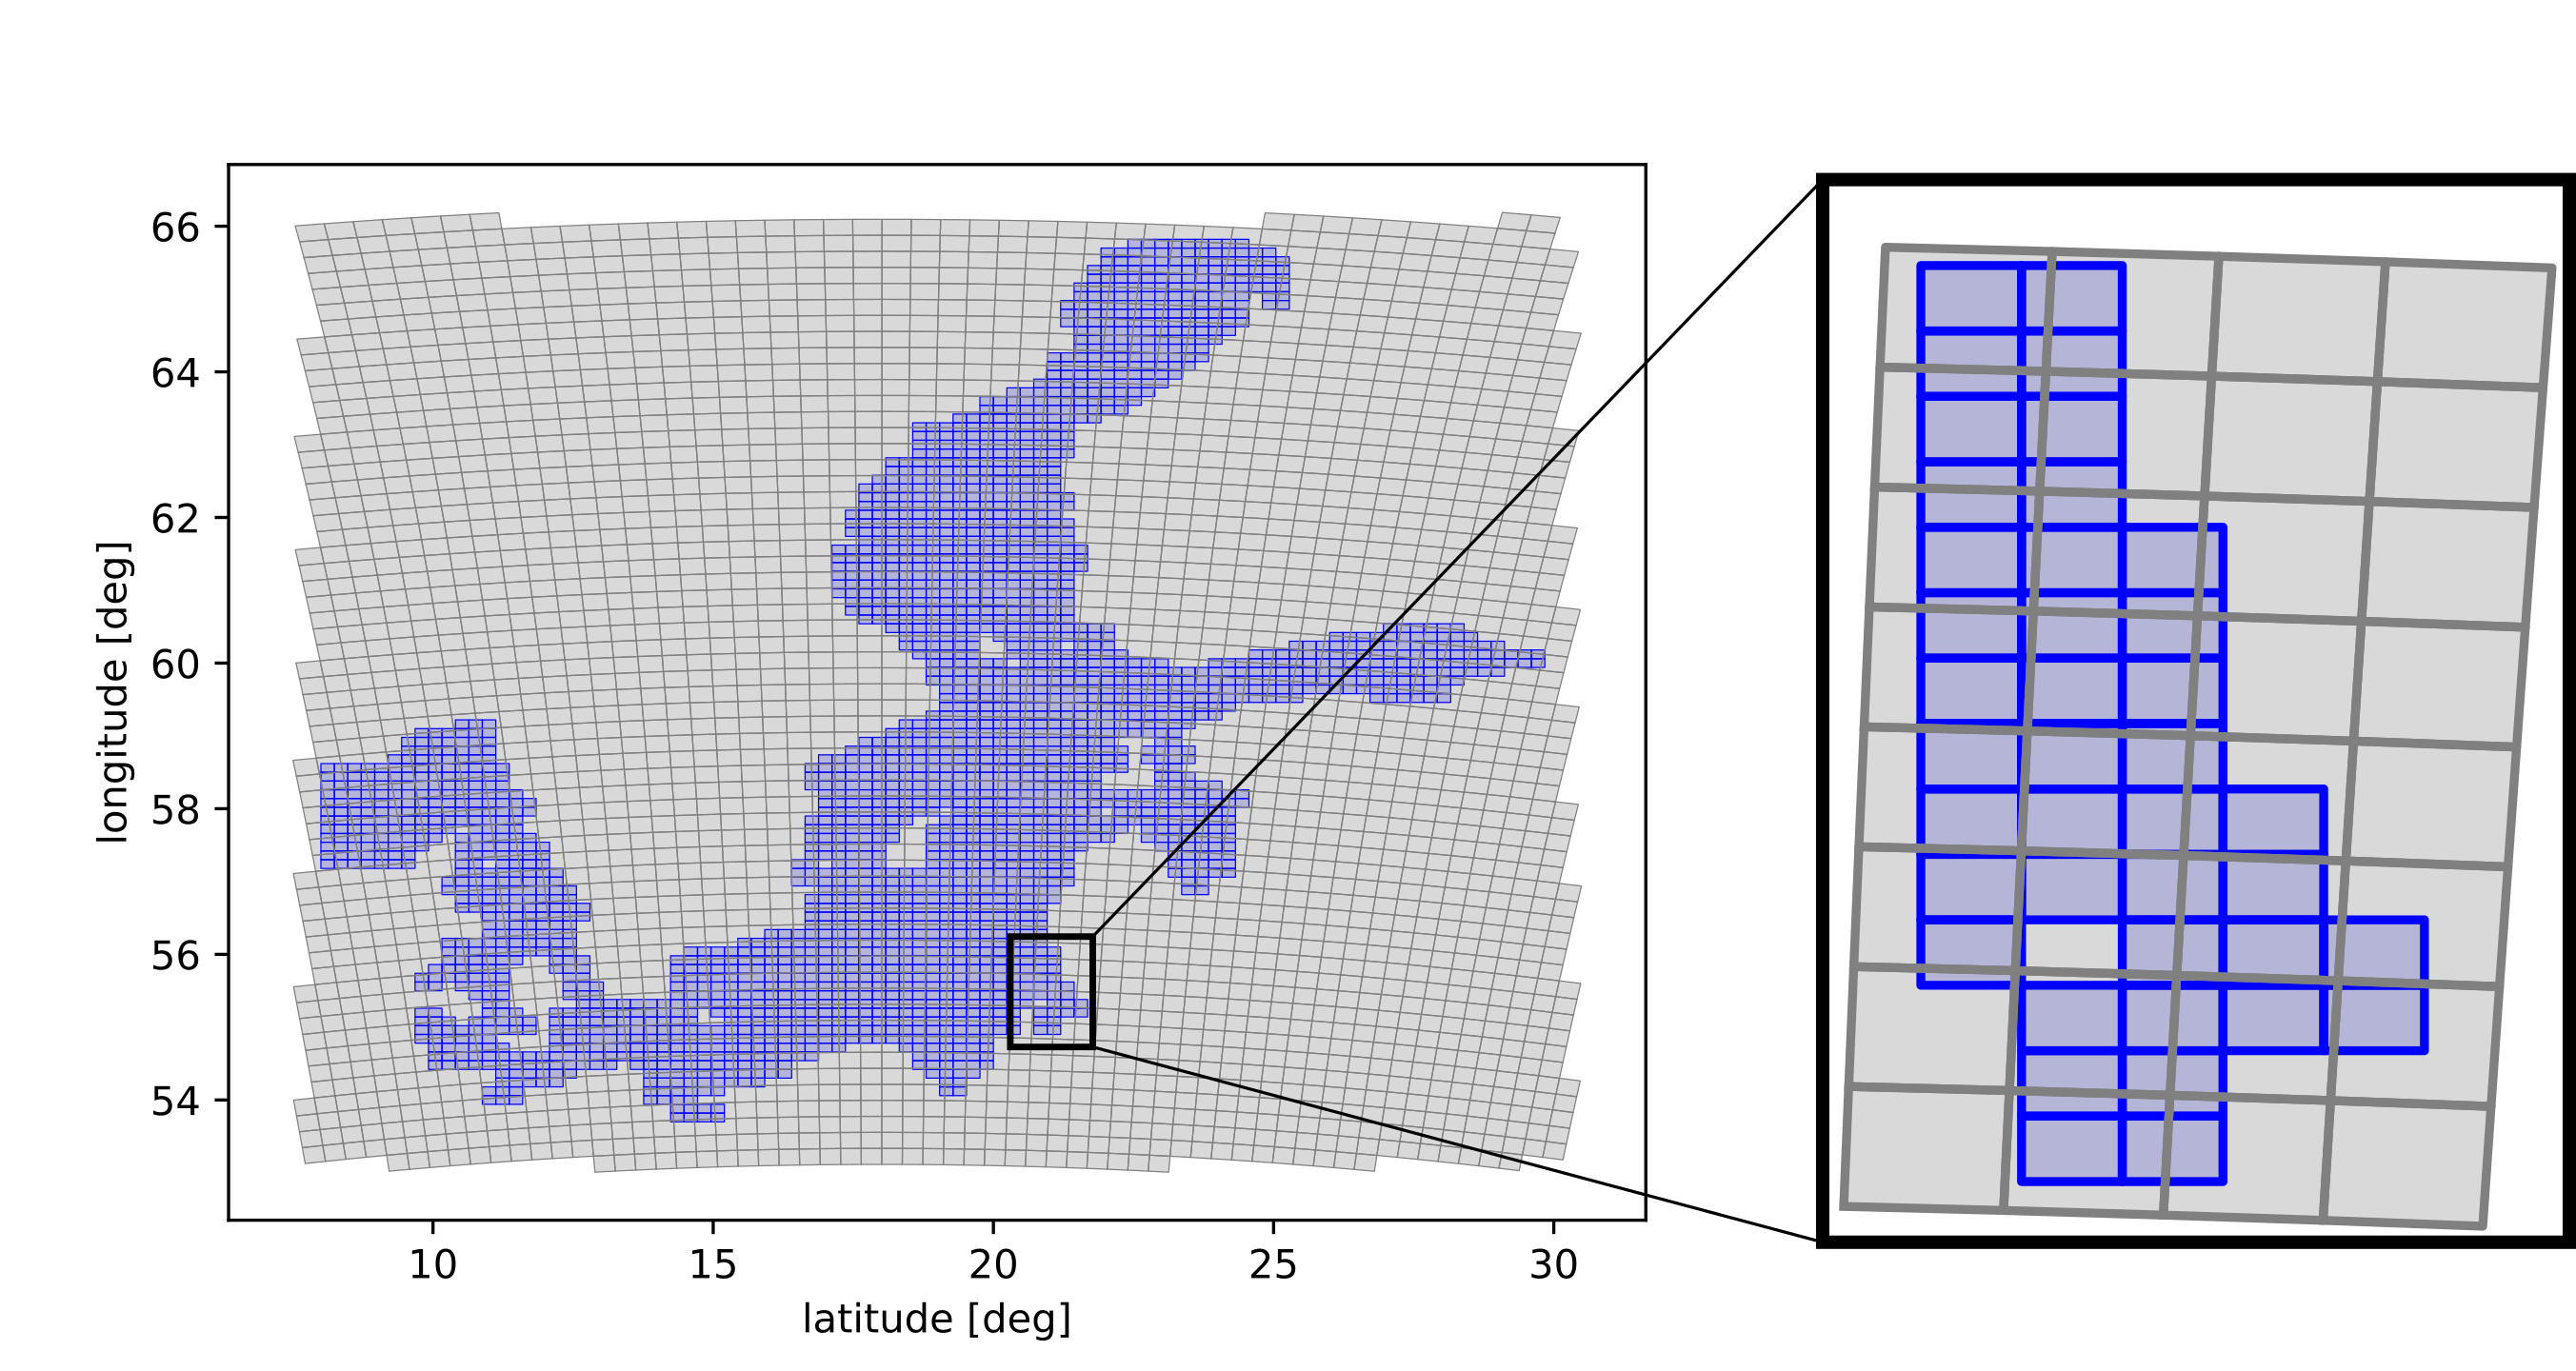
\includegraphics[width=\linewidth]{"./figures/grids.pdf"} 
		\caption{
		\label{fig:grids2D}
		Overlaying grids of atmospheric and ocean model for the Baltic Sea.
		}
		\end{subfigure}
    \hfill
    \vspace{1em}
    \begin{subfigure}[t]{0.48\textwidth}
        \centering
		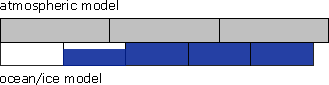
\includegraphics[width=\linewidth]{"./figures/grids1D.pdf"}
		\caption{
		\label{fig:grids1D}
		Abstraction of figure \ref{fig:grids2D} in one spatial horizontal dimension. Bottom model can support different surface types as water (blue) and ice (white).
		}
	\end{subfigure}
	\caption{The different grids of the different models.}
\end{figure}

To exemplify this problem let us consider the calculation of a flux of something from the atmosphere to the bottom.
%
Usually, if the flux depends on the state of the ocean, some state variables have to be communicated first to the atmosphere.
%
Since the atmospheric grids are normally larger, the information has to be averaged (weighted by areas) over several bottom cells, 
over different surface types, see \Fig{fig:conservative_mapping1}.

With this averaged state information and its own internal state, the atmospheric model can now calculate the flux as a field on the atmospheric grid.
%
It is noteworthy that the flux cannot be calculated for the different surface types differently, since the atmospheric model does not know about that (at least not without changing the code significantly).
%
Finally, the flux field then has to be redistributed on the bottom cells (again in a area-weighted manner such that flux variable is overall conserved), 
see \Fig{fig:conservative_mapping2}.
%
Since the flux is only calculated from averaged information and not surface-type-dependent, this approach locally not consistent and can become inaccurate. 
%
This is especially true if many bottom grid cells are covered by one atmospheric grid cell.

\begin{figure}[H]
	\centering
    \begin{subfigure}[t]{0.48\textwidth}
        \centering
		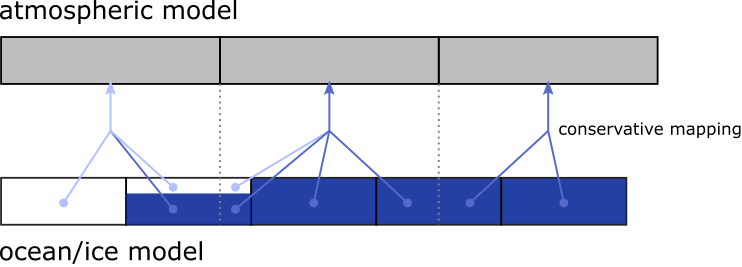
\includegraphics[width=\linewidth]{"./figures/conservative_mapping1.pdf"} 
		\caption{
		\label{fig:conservative_mapping1}
		Average of ocean's state variables communicated to the atmosphere.
		}
		\end{subfigure}
    \hfill
    \begin{subfigure}[t]{0.48\textwidth}
        \centering
		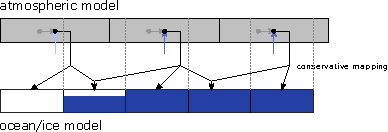
\includegraphics[width=\linewidth]{"./figures/conservative_mapping2.pdf"}
		\caption{
		\label{fig:conservative_mapping2}
		Calculation of fluxes in the atmospheric model and remapping on to the ocean's grid.
		}
	\end{subfigure}
	\caption{The standard way of coupling.}
\end{figure}

The alternative approach chosen within the IOW ESM is the introduction of a third component, i.e. the flux calculator that acts on the exchange grid.
%
This grid is the set of intersections between the atmospheric and the bottom grid and thus has, by construction, 
a higher resolution than all involved model components, see \Fig{fig:grids1D_plus_exchange}.

\begin{figure}[H]
	\centering
	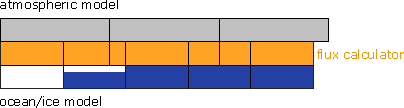
\includegraphics[width=0.48\linewidth]{"./figures/grids1D_plus_exchange.pdf"} 
	\caption{
	\label{fig:grids1D_plus_exchange}
	Introduction of the exchange grid on which the flux calculator is acting.
	}
\end{figure}

The example from above, i.e. a flux shall be communicated from the atmosphere to the ocean, is then treated as follows.

First, the physical components of the coupled model send their necessary state variables to the flux calculator. 
%
The variables are thereby mapped onto the exchange grid, see \Fig{fig:exchange_grid_mapping1}.
%
Importantly, since the exchange-grid cells are always smaller or equal to the „physical“ grid cells, this mapping does not feature any averaging and,
%
thus, no information is lost.
%
Moreover, different surface types can be treated individually since the flux calculator might know about these feature of the bottom model.

Second, with all the state information, the flux calculator is now able to calculate the flux of interest.
%
Any formula can be used that maps the given state variables onto the desired flux field. 
%
The calculation only requires local information and can be surface-type-dependent.
%
The resulting flux has to be finally mapped onto the bottom grid, see \Fig{fig:exchange_grid_mapping2}.
% 
Note that, although not shown in the figures, the very same fluxes are communicated to the atmospheric model as well.
%
This ensures a conservative and consistent exchange of mass, energy and momentum between the different model components. 

\begin{figure}[H]
	\centering
    \begin{subfigure}[t]{0.48\textwidth}
        \centering
		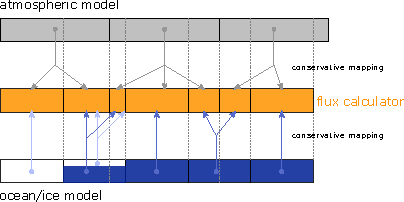
\includegraphics[width=\linewidth]{"./figures/exchange_grid_mapping1.pdf"} 
		\caption{
		\label{fig:exchange_grid_mapping1}
		Communication of state variables to the flux calculator. Importantly no averaging is performed while mapping.
		}
		\end{subfigure}
    \hfill
    \begin{subfigure}[t]{0.48\textwidth}
        \centering
		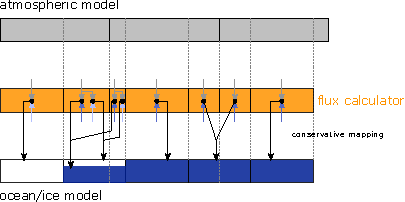
\includegraphics[width=\linewidth]{"./figures/exchange_grid_mapping2.pdf"}
		\caption{
		\label{fig:exchange_grid_mapping2}
		Fluxes are calculated and subsequently communicated to the bottom model.
		}
	\end{subfigure}
	\caption{Coupling the models via the exchange grid and the flux calculator.}
\end{figure}

%%%%%%%%%%%%%%%%%%%%%%%%%%%%%%%%%%%%%%%%%%%%%%%%%%%%%%%%
% SECTION: Coupling concept                            %
%%%%%%%%%%%%%%%%%%%%%%%%%%%%%%%%%%%%%%%%%%%%%%%%%%%%%%%%
\section{Current implementation of the coupling concept}

\subsection{Components}
The following components can be coupled in the IOW ESM:
\begin{itemize}
\item \textbf{COSMO-CLM} atmospheric model, see \href{https://wiki.coast.hereon.de/clmcom/}{here}
\item \textbf{MOM5.1} ocean model (including (a) ERGOM ecosystem model and (b) dynamic ice model coupled internally via FMS coupler), see \href{https://mom-ocean.github.io/}{here}
\end{itemize}

\subsection{Coupling philosophy}
The components are coupled via the OASIS3-MCT coupler (see \href{https://oasis.cerfacs.fr/en/}{here}), but not directly:
\begin{enumerate}
\item The components (Atmosphere, Land, Ocean) communicate their variables (temperature, pressure, velocity etc.) to a \textbf{flux calculator} executable.
\item The \textbf{flux calculator} runs on an exchange grid and calculates  fluxes (radiation, heat, mass, momentum).
\item The fluxes are back-communicated to the components (Atmosphere, Land, Ocean).
\end{enumerate}
This procedure automatically ensures conservation of all exchanged quantities.

\begin{center}
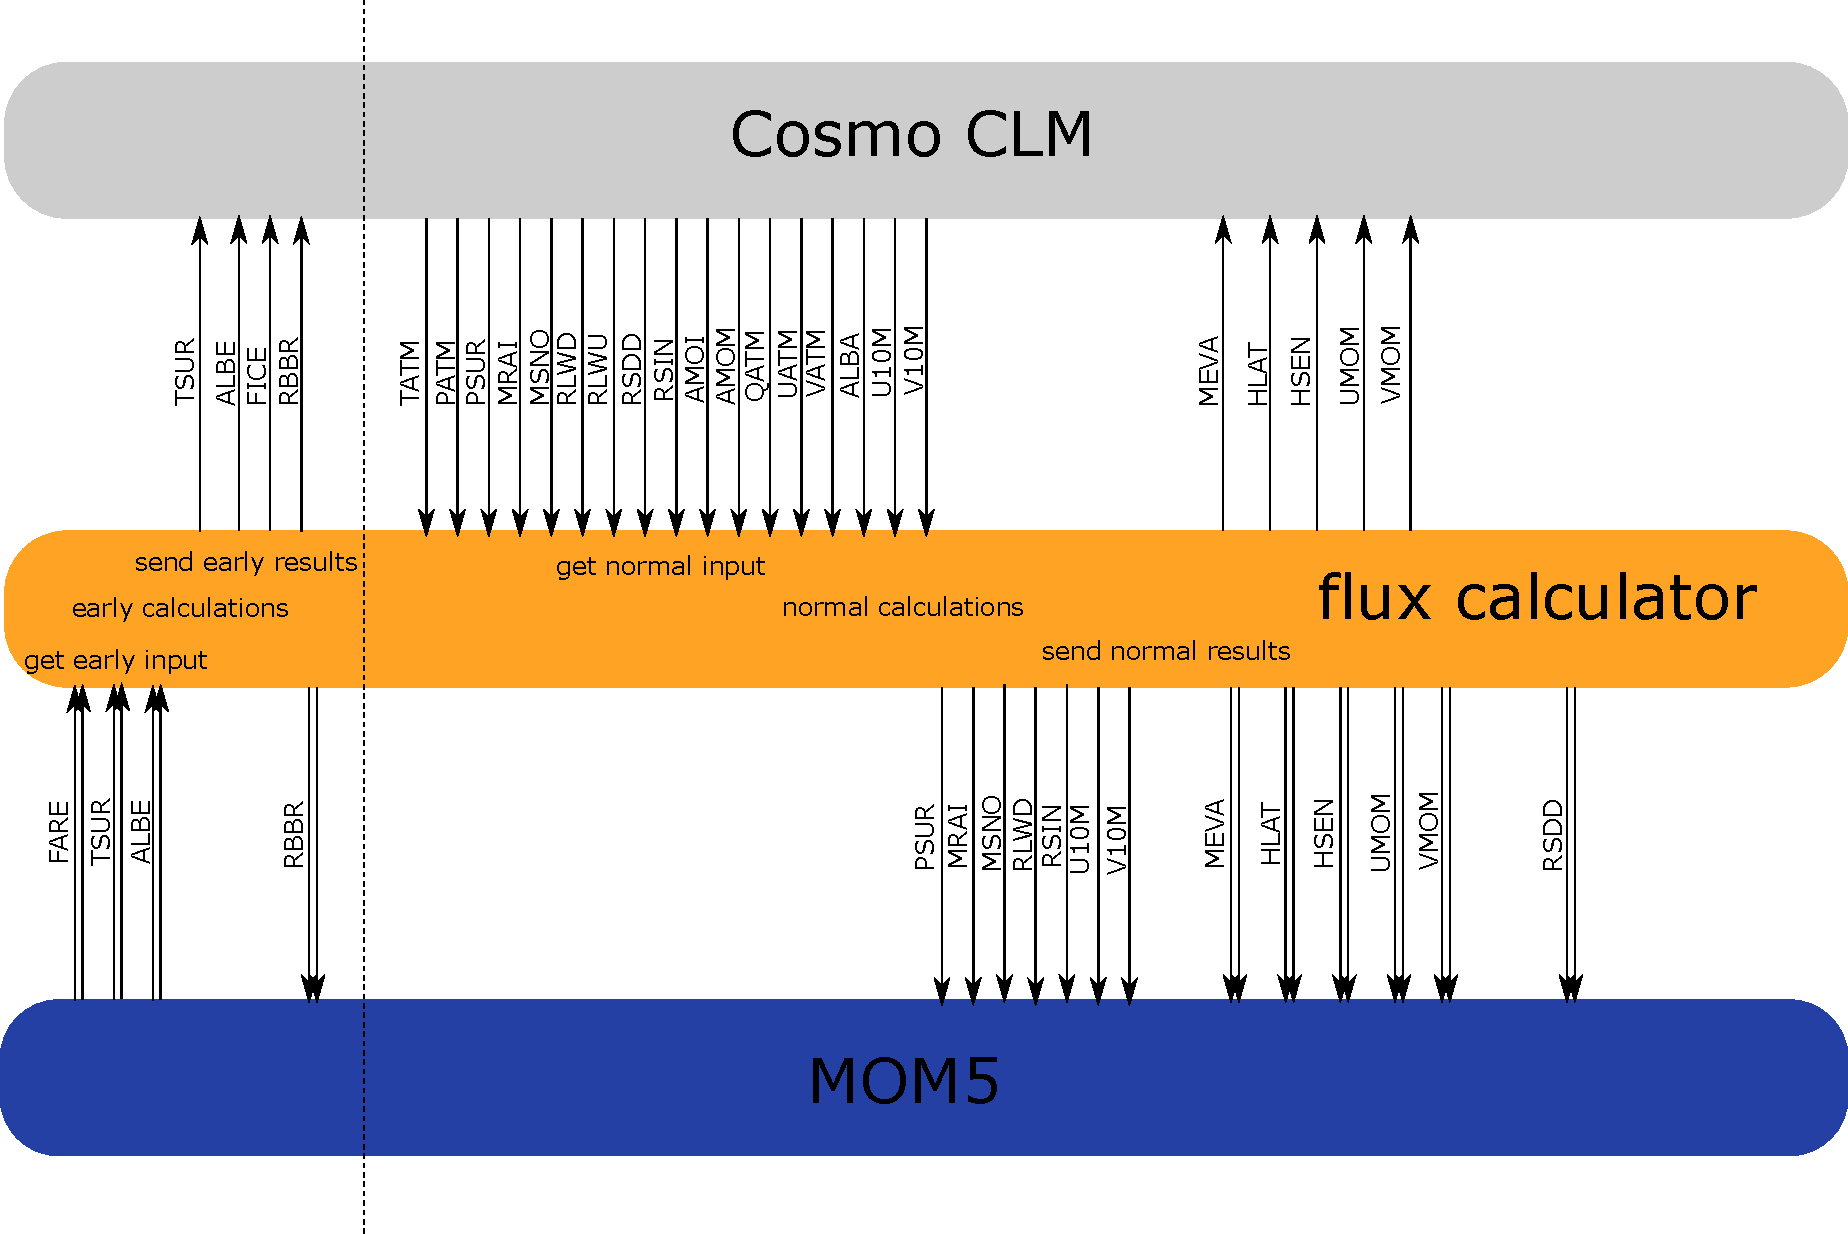
\includegraphics[scale=0.3]{./figures/sequence-diagram.pdf}
\end{center}

Some fluxes, however, do not fit into this concept. Precipitation and radiative fluxes will still be determined by the atmospheric model (on the coarse atmospheric grid) and the resulting fluxes will be sent to the flux calculator executable. Precipitation is then simply passed to the bottom models. Radiative fluxes need some redistribution between different surface areas under the same atmospheric grid cell (e.g. ocean and land) that show different albedo. This concept is described in detail in Section~\ref{sec:fluxes_radiation}.

Still, there is no direct communication the two physical components and this enables ultimately interchangeability of the models.

%%%%%%%%%%%%%%%%%%%%%%%%%%%%%%%%%%%%%%%%%%%%%%%%%%%%%%%%%%%%%%%%
% SECTION: Design and structure of the IOW ESM project  %
%%%%%%%%%%%%%%%%%%%%%%%%%%%%%%%%%%%%%%%%%%%%%%%%%%%%%%%%%%%%%%%%
\newpage
\section{Design and structure of the IOW ESM project}

\begin{figure}[H]
	\centering
	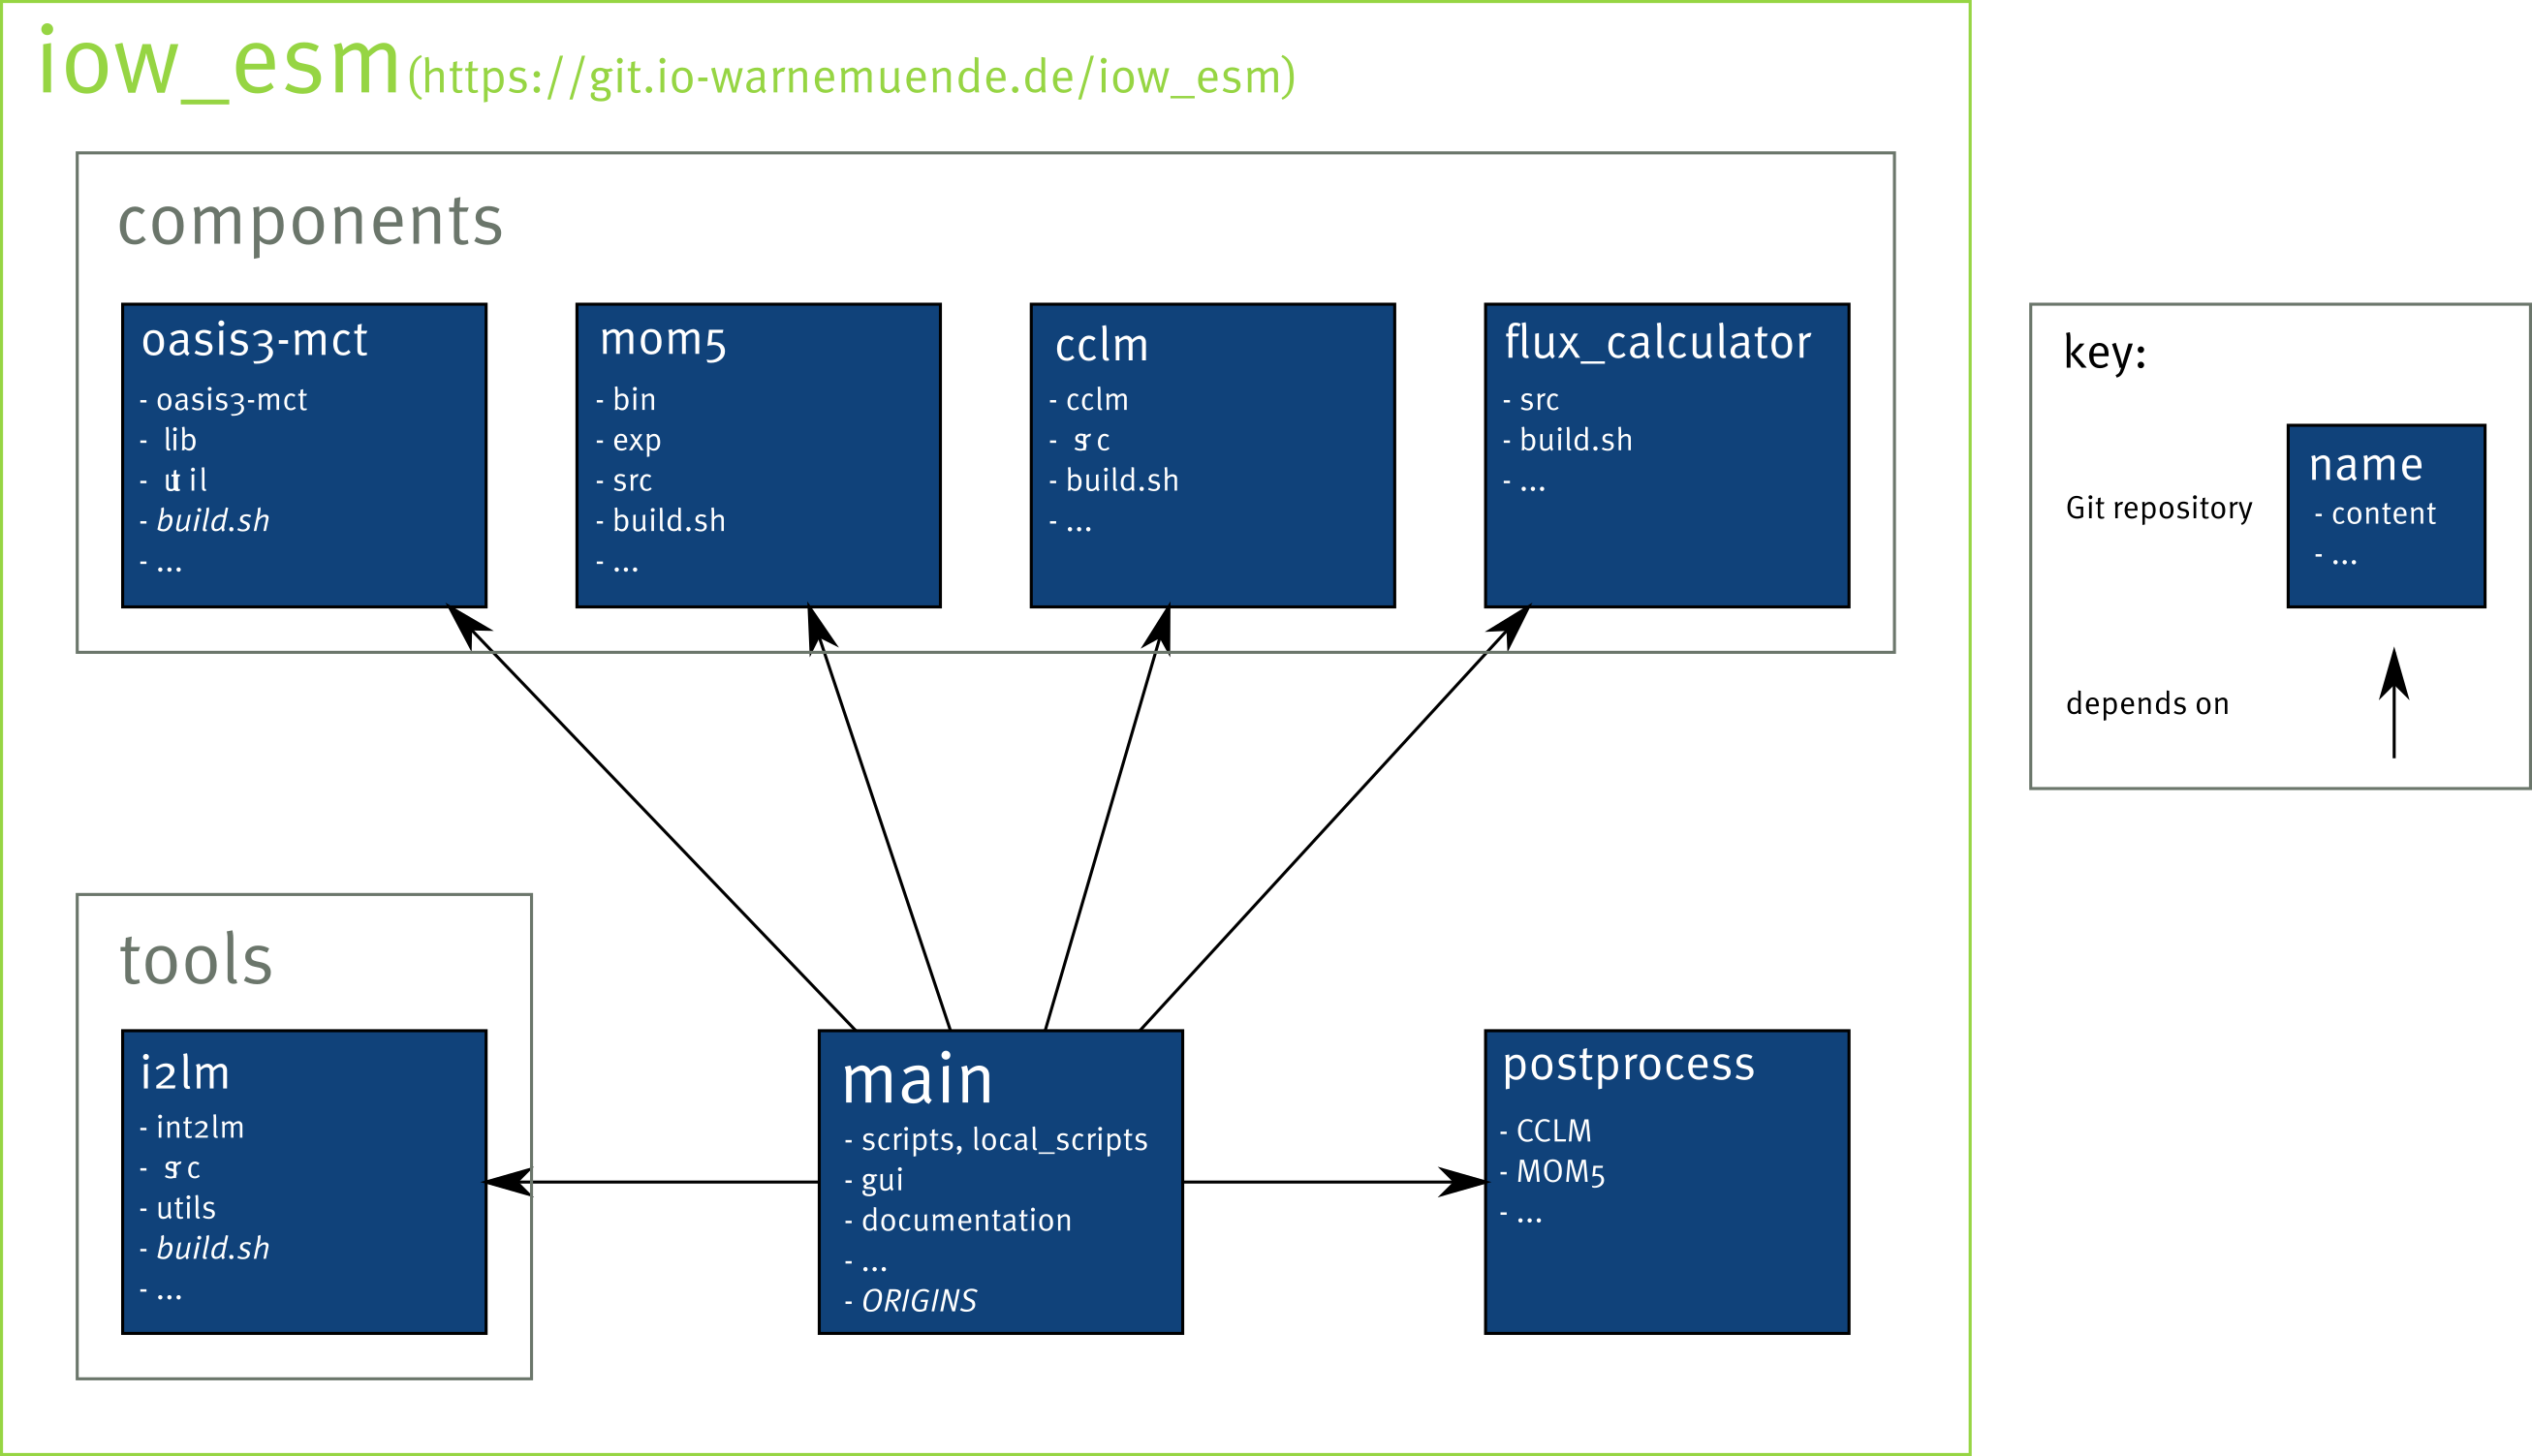
\includegraphics[width=\linewidth]{"./figures/project_structure.pdf"} 
	\caption{Structure of the project's source code management.}
\end{figure}

%%%%%%%%%%%%%%%%%%%%%%%%%%%%%%%%%%%%%%%%%%%%%%%%%%%%%%%%%%%%%%%%
% SECTION: Getting and setting up the IOW ESM for first usage  %
%%%%%%%%%%%%%%%%%%%%%%%%%%%%%%%%%%%%%%%%%%%%%%%%%%%%%%%%%%%%%%%%
\newpage
\section{Getting and setting up the IOW ESM for first usage}

How to get the sources of the IOW ESM and setting it up for a first run is described in the \Readme file.

Once the steps described therein have been followed, the user finds a directory structure that is presented in \Sec{sec:directory-structure}. 


%%%%%%%%%%%%%%%%%%%%%%%%%%%%%%%%%%%%%%%%%%%%%%%%%%%%%%%%
% SECTION: Directory structure of the IOW ESM          %
%%%%%%%%%%%%%%%%%%%%%%%%%%%%%%%%%%%%%%%%%%%%%%%%%%%%%%%%
\section{Directory structure of the IOW ESM}
\label{sec:directory-structure}
Under a base directory which the user can select, there is the following directory structure:
\begin{verbatim}
components
   OASIS3-MCT
   CCLM
   MOM5
   flux_calculator
tools
   I2LM
input
   CCLM_MAINGRID
   MOM5_MAINGRID
   GETM_SUBGRID
scripts
   prepare
   run
postprocess
   MOM5
      task1
      task2
      ...
   CCLM
      task1
      task2
      ...
work
   CCLM_MAINGRID
   MOM5_MAINGRID
   GETM_SUBGRID
output
   RUN01
      CCLM_MAINGRID
         19500101
         19510101
         ...
      MOM5_MAINGRID
         ...
      GETM_SUBGRID
         ...
   RUN02
   ...
hotstart
   RUN01
      CCLM_MAINGRID
         19510101
         19520101
         ...
      MOM5_MAINGRID
         ...
      ...
   RUN02
   ...
\end{verbatim}

\subsection{The components directory}
This directory contains the components of the IOW-ESM, which are
\begin{itemize}
\item \textbf{COSMO-CLM}, a regional atmospheric model
\item \textbf{MOM5}, a hydrodynamic ocean model
\item the \textbf{OASIS3-MCT} library for coupling the components via MPI
\item the \textbf{flux calculator}, a separate executable to calculate fluxes between atmosphere and ocean/land on an exchange grid.
\end{itemize}

Each component's directory contains subdirectories for
\begin{itemize}
\item the source code,
\item the compile scripts,
\item the compiled libraries and/or executables.
\end{itemize}

Note that all components depend on the OASIS3-MCT library but not mutually on each other.

\subsection{The tools directory}
This directory contains components of the IOW-ESM that are not directly coupled to other components but provide useful input for the models.
Currently the following tools are available
\begin{itemize}
\item \textbf{int2lm}, a part of the CCLM package to generate forcings from coarse data, see \href{https://wiki.coast.hereon.de/clmcom/}{here}
\end{itemize}
 

\subsection{The input directory}
The user of the model system has to create a directory called \texttt{input}.
It contains subdirectories for the individual model instances which shall be coupled.
For each model instance, the subdirectory shall be named \texttt{\color{red}MODELNAME\color{black}\_\color{red}GRIDNAME} where \texttt{\color{red}MODELNAME} is the name of the model (as it is called in the \texttt{components} folder) and \texttt{\color{red}GRIDNAME} is the name of the model grid, since more than one instance of a model can run at the same time but with different grids.
Section~\ref{sec:preparing_input_folders} describes how to store model input in these folders.

In addition, there are three files directly in the \texttt{input} directory:
\begin{itemize}
\item \texttt{global\_settings.py} contains settings for the entire model system, such as name and duration of the present run, coupling timestep, or whether the work directory in which the coupled model runs should be global or node-local.
\item \texttt{flux\_calculator.nml} is a configuration file for the \texttt{flux\_calculator} executable which defines how fluxes between atmosphere and land/sea shall be calculated, i.e. which bulk formulae are used.
\item \texttt{namcouple} is the OASIS3-MCT coupling configuration file and describes how data are exchanged between the model subcomponents. It needs to match the configuration in \texttt{flux\_calculator.nml}. It can be thus generated automatically by setting the option \texttt{generate\_namcouple = True} in \texttt{global\_settings.py}. Importantly, for an uncoupled run you have to provide a \texttt{namcouple} file with \texttt{\$NFIELDS} equal to zero. 
\end{itemize}

\subsection{The scripts directory}
This directory contains scripts (bash or python3 scripts) which perform tasks in preparing model runs, running the model system, or 

\subsection{The postprocess directory}
This directory contains scripts (bash and python) for postprocessing of data which is located in the output directory.

\subsection{The work directory (automatically created during model start)}
This is the directory in which the models are actually executed.
It can also be located in another place, such as a RAM drive.
If the model run fails, you can check for errors here.

\subsection{The output directory (automatically created during model run)}
For each run of the model system, there will be a separate directory which contains the model results.
These are sorted by sub-model and by starting time.

\subsection{The hotstart directory (automatically created during model run)}
This contains hotstart files to restart the model from a specific date.
The directory is sorted like the \texttt{output} folder.


%%%%%%%%%%%%%%%%%%%%%%%%%%%%%%%%%%%%%%%%%%%%%%%%%%%%%%%%
% SECTION: Compiling IOW ESM components                %
%%%%%%%%%%%%%%%%%%%%%%%%%%%%%%%%%%%%%%%%%%%%%%%%%%%%%%%%
\newpage
\section{Compiling IOW ESM components}

It is important to compile the OASIS3-MCT libraries first before compiling the other subcomponents.
This is even true if you want to build only the CCLM or the MOM5, respectively, for an uncoupled run.
Whether a model runs coupled or uncoupled is only decided via the configuration files in the `input` directory, see \Sec{sec:preparing_input_folders}.
The binaries are the same for both types of applications.

The correct order of building is ensured by using the \texttt{build.sh} script in the base directory.
How this script is called correctly is written in detail in the \Readme file.

However, it is still possible to build each component individually.
In order to compile one of the components, go to the corresponding folder:
\begin{itemize}
\item \texttt{components/OASIS3-MCT}
\item \texttt{components/CCLM}
\item \texttt{components/MOM5}
\item \texttt{components/flux\_calculator}
\end{itemize}
This folder contains the source code and makefiles required to build this component.
Execute the file \texttt{build.sh}, which will then create your executable.
How this script is called correctly is written in detail in the \Readme file.
You will need to modify the file \texttt{build.sh} according to the machine you are compiling it on, and according to the compiler and MPI libraries which you want to use.
For some machines that are typically used at the IOW the working build scripts are already provided in the repository.
Which machines are supported and which steps you have to follow to register a new machine is written in detail in the \Readme file.

For compiling in debug mode (with traceback), the build scripts can be called with an additional argument which will create a separate executable with debug options enabled. You can define which of the executables to use by specifying \texttt{debug\_mode = True} or \texttt{False} in the file \texttt{global\_settings.py}. You should obviously not do productions runs with the debug-mode executables since this will waste computational resources.


%%%%%%%%%%%%%%%%%%%%%%%%%%%%%%%%%%%%%%%%%%%%%%%%%%%%%%%%
% SECTION: Preparing IOW ESM runs                      %
%%%%%%%%%%%%%%%%%%%%%%%%%%%%%%%%%%%%%%%%%%%%%%%%%%%%%%%%
\newpage
\section{Preparing IOW ESM runs}
\subsection{Preparing the input folders for individual models}
\label{sec:preparing_input_folders}

The IOW ESM supports to run a single atmospheric model and several ocean or land models at the same time.
For each of these, a sub-folder in the \texttt{input} directory has to be prepared.
It shall be named \texttt{\color{red}MODELNAME\color{black}\_\color{red}GRIDNAME} where \texttt{\color{red}MODELNAME} is the name of the model (as it is called in the \texttt{components} folder) and \texttt{\color{red}GRIDNAME} is the name of the model grid.

% TODO: upload (small) example setups to some website
%To start, it makes most sense to download existing example \texttt{input} folders from this webpage: 
%\color{red}\url{https://www.io-warnemuende.de/???}\color{black}

If you work on the machines typically used at the IOW, the \Readme file explains in detail how and where to get working example setups.

\subsubsection{General remarks}
The input folders can contain files and arbitrarily named sub-directories which will simply be copied (or dynamically linked) to create a work directory for the model.
An exception are subfolders named \texttt{from}.
These should themselves contain subfolders named after years or dates as YYYYMMDD (e.g. \texttt{1950} or \texttt{19501201}).
In case that the starting date of a model run is equal to or larger than a subfolder's date, the files inside this folder will be copied to the directory containing the folder \texttt{from}.
For example, if there are files
\begin{verbatim}
input/MOM5_maingrid/OBC/from/1950/obc_sealevel.nc
input/MOM5_maingrid/OBC/from/1951/obc_sealevel.nc
input/MOM5_maingrid/OBC/from/1952/obc_sealevel.nc
\end{verbatim}
and the starting date of a model run is 1951-06-01, the file\\ 
\texttt{input/MOM5\_maingrid/OBC/from/1951/obc\_sealevel.nc}\\
will be copied (or linked) to \\
\texttt{work/MOM5\_maingrid/OBC/obc\_sealevel.nc}.

\subsubsection{Expected contents of the COSMO-CLM input directory}
The following settings are required in \texttt{INPUT\_PHY}:\\
\texttt{llake = .FALSE.}\\
\texttt{lseaice = .FALSE.}

For a coupled run the following settings are required in the \texttt{OASISCTL} block of \texttt{INPUT\_OASIS}:\\
\texttt{ytype\_lsm = 'terra',}\\
\texttt{ytype\_oce = 'flxcl',}\\
\texttt{CPL\_FLG  = 1,}\\
\texttt{dt\_cp = *auto*}
 
whereas for an uncoupled run it is mandatory to have\\
\texttt{ytype\_oce = 'nooce'}

The following settings are required in \texttt{INPUT\_DYN}:\\
\texttt{l2tls = .TRUE.}

\subsubsection{Expected contents of a MOM5 input directory}
For a coupled run the following settings in the \texttt{coupler\_nml} block of \texttt{input.nml} are required
\texttt{dt\_cpld  = *AUTO*} \\
\texttt{dt\_atmos = *AUTO*} \\
\texttt{do\_atmos = .false.} \\
\texttt{do\_land = .false.} \\
\texttt{do\_ice = .true.} \\
\texttt{do\_ocean = .true.} \\
\texttt{type\_atmos = 'flux\_calculator'}

whereas for an uncoupled run it is mandatory to have
\texttt{type\_atmos = 'none'}

\subsection{Preparing the global settings}

\subsubsection{Modeller's information}
\begin{verbatim}
####################################################
# Global settings for the IOW-ESM model run        #
####################################################

###################################
# STEP 1: Info about the modeller #
###################################
modeller        = "Sven Karsten"                                               # name of the modeller who is responsible
email           = "sven.karsten@io-warnemuende.de"                             # contact of the responsible modeller
institution     = "Leibniz Institute for Baltic Sea Research Warnemunde (IOW)" # name of the institute
\end{verbatim}


\subsubsection{Run information}

\begin{verbatim}
###############################
# STEP 2: Info about the run  #
###############################
run_name        = "RUN14"        # name of the current run
run_description = "run for fixing land-sea mask issue"     # description: what is this run good for?
init_date       = "19800101"           # date when model is/was cold-started
final_date      = "20100101"           # when will the model run finally end? (YYYYMMDD) 
                                       # choose final_date<init_date to make model run as long as forcing is available
debug_mode      = False                # whether or not to use executables compiled with debugging options (slow)

#################################################
# STEP 3: Time stepping info                    #
#################################################
coupling_time_step = 600               # time step when fluxes are calculated and exchanged (s)
run_duration = "1 month"                # duration of one model run (day/days, month/months, year/years)
runs_per_job = 1                       # how many runs will be done in one job script
max_attempts = 1                       # if a run fails, you can have new attempts with modified settings

#################################################
# STEP 4: Working directory options             #
#################################################
workdir_base = "work"                  # base directory where individual model work dirs are located. 
                                       # if it does not start with "/", it is interpreted relative to IOW_ESM_ROOT
local_workdir_base = "${LOCAL_TMPDIR}"                # If you want the workdirs to be created locally on the nodes, give an absolute path here.
                                       # This can also be an environment variable, e.g. "${LOCAL_TMPDIR}".
copy_to_global_workdir = True          # If local_workdir_base is given, use this flag to specify whether the 
                                       # entire content of the local workdir will be copied to workdir_base.
                                       # Output and restarts will be collected anyway.
link_files_to_workdir = True           # TRUE: input files will be linked to the working directory.
                                       # FALSE: input files will be copied to the working directory.

################################################
# STEP 5: Two-way coupling options             #
################################################
flux_calculator_mode = "single_core_per_bottom_model"   # "single_core_per_bottom_model": For each bottom model, one instance of flux_calulator will be
#flux_calculator_mode = "none"                           # started in an MPI task on its own core.
                                                        # "on_bottom_model_cores": (not available yet) The flux_calculator executable runs on the 
                                                        # same cores as the bottom models while they wait (some sort of hyperthreading).
                                                        # "none": no flux_calculator executable is started

################################################
# STEP 6: Parallel execution options           #
################################################
mpi_run_command = 'mpirun -configfile mpmd_file'        # the shell command used to start the MPI execution described in a configuration file "mpmd_file"
                                                        # it may contain the following wildcards that will be replaced later:
                                                        #   _NODES_ total number of nodes
                                                        #   _CORES_ total number of cores to place threads on
                                                        #   _THREADS_ total number of mpi threads
                                                        #   _CORESPERNODE_ number of cores per node to use
                                                        #   Examples: Intel MPI: 'mpirun -configfile mpmd_file'
                                                        #             OpenMPI  : 'mpirun --app mpmd_file'
mpi_n_flag = '-n'                                       # the mpirun flag for specifying the number of tasks.
                                                        #   Examples: Intel MPI: '-n'
                                                        #             OpenMPI  : '-np'
bash_get_rank = 'my_id=${PMI_RANK}'                     # a bash expression that saves the MPI rank of this thread in the variable "my_id"
                                                        #   Examples: Intel MPI    : 'my_id=${PMI_RANK}'
                                                        #             OpenMPI+Slurm: 'my_id=${OMPI_COMM_WORLD_RANK}'
python_get_rank = 'my_id = int(os.environ["PMI_RANK"])' # a python expression that saves the MPI rank of this thread in the variable "my_id"
                                                        #   Examples: Intel MPI    : 'my_id = int(os.environ["PMI_RANK"])'
                                                        #             OpenMPI+Slurm: 'my_id = int(os.environ["OMPI_COMM_WORLD_RANK"])'
cores_per_node = 40                                     # maximum number of cores per node that shall be used
jobscript_template = 'input/jobscript_hlrng'            # path to a template file which will become the job script to run the model
                                                        # may contain the same wildcards as mpi_run_command, plus _IOW_ESM_ROOT_
check_layout_only = True                                # if set to True, will not run the models but only print which model runs on which node

resubmit_command = "source ~/.bash_profile; sbatch jobscript" # will be executed in 'scripts/run'

################################################
# STEP 7 (optional): generate namcouple file automatically  #
################################################
generate_namcouple = True

################################################
# STEP 8 (optional): Start postprocessing after run has finished #
################################################
process_raw_output = True
\end{verbatim}

\subsection{Preparing a jobscript template}

In order to start a run of the IOW ESM on a supercomputer, a jobscript template must be provided.
If you have deployed your setup as described in the \Readme file, you will have such a template in the \texttt{input} directory.
This has to be adapted to your personal needs as follows.

\begin{sloppypar}
\begin{enumerate}
%\item Specify the parallelization layout of individual models as described in the component-specific subsections.
\item Be sure that you leave the following lines unchanged \\
\texttt{\#SBATCH --nodes=\_NODES\_}\\
\texttt{\#SBATCH --ntasks=\_CORES\_}\\
\texttt{\#SBATCH --tasks-per-node \_CORESPERNODE\_}\\
These will be filled later by the run scripts according to the parallelization layout.
\item Adjust the job name, the account, the compute partition and the runtime.
\item Go to the file \texttt{input/global\_settings.py} and specify the filename of your template via the variable \texttt{jobscript\_template}
\item Also in \texttt{input/global\_settings.py}, fill in the number of cores per node to use.
%\item Go to the folder \texttt{scripts/prepare} and run \texttt{python3 create\_jobscript.py}, which will take the supercomputer-specific job script defined in \texttt{input/global\_settings.py} and produce a file \texttt{scripts/run/jobscript} by filling in in the required number of cores and nodes for the full coupled model.
\item Later you may want to check whether the parallelization is efficient, i.e. whether none of the components has too much idle time waiting for the others. 
This is described in \Sec{sec:optimizing}
\item The actual jobscript is then automatically generated (via the script \texttt{scripts/prepare/create\_jobscript.py}) when you start a run.
\end{enumerate}
\end{sloppypar}

\subsection{Defining the parallelization layout}
Parallelization is defined for each individual model, as described in the following subsections.
The parallelization of the entire model system will then be derived from these individual settings automatically when you start a run.

\subsubsection{Defining CCLM parallelization}
CCLM uses a rectangular parallelization in X and Y direction, where X and Y are the zonal and meridional direction on the rotated lat-lon grid. 
The number of rectangles in each direction can be specified in the file \texttt{input/CCLM\_\color{red}???\color{black}/INPUT\_ORG}.
This information will be automatically used by the script \texttt{/scripts/prepare/get\_parallelization\_layout.py}.


\subsubsection{Defining MOM5 parallelization}
MOM5 uses a rectangular decomposition defined in \texttt{input.nml}. 
A file named \texttt{mask\_table} can be used to define which of the rectangles contain land points only.
MOM5 comes with a tool to find out parallelization layouts which optimize the relative fraction of these land domains.
This information will be automatically used by the script \texttt{/scripts/prepare/get\_parallelization\_layout.py}.

We recommend to use the same layout for both ocean model and ice model.


\subsection{Generating the exchange grid}
To create the exchange grid

\subsection{Creating the coupling namelists}

\subsubsection{Time stepping options}

\begin{verbatim}
  !!!!!!!!!!!!!!!!!!!!!!!!!!!!!!!!!!!!!!!!!!!!!!!!!!!!!!!!!
  ! time stepping options - will be changed automatically !
  !!!!!!!!!!!!!!!!!!!!!!!!!!!!!!!!!!!!!!!!!!!!!!!!!!!!!!!!!
  timestep      = *auto*,   ! coupling time step in seconds
  num_timesteps = *auto*,
  
  verbosity_level = 1,		! 2 - debug, 1 - standard, 0 - error
  
  name_atmos_model = 'CCLM_Eurocordex'
\end{verbatim}

\subsubsection{Input from bottom models}

\begin{verbatim}
  !!!!!!!!!!!!!!!!!!!!!!!!!!!!!!!!!!!!!!!!!
  ! Input from bottom models              !
  ! by (model,surface_type,runningnumber) !
  !!!!!!!!!!!!!!!!!!!!!!!!!!!!!!!!!!!!!!!!!
  !name_bottom_var_t(1,1:6,1) = 'FARE','none','none','none','none','none',        ! which variables (model,surface_type,runningnumber) come from the bottom model grid
  name_bottom_var_t(1,1:6,1) = 'FARE','FARE','FARE','FARE','FARE','FARE',        ! which variables (model,surface_type,runningnumber) come from the bottom model grid
  name_bottom_var_t(1,1:6,2) = 'TSUR','TSUR','TSUR','TSUR','TSUR','TSUR',  
  name_bottom_var_t(1,1:6,3) = 'FICE','FICE','FICE','FICE','FICE','FICE',
  val_bottom_var_t (1,1:6,3) = 0.0, 1.0, 1.0, 1.0, 1.0, 1.0,                     ! constant values can be given, in this case no read from coupler
  name_bottom_var_t(1,1:6,4) = 'ALBE','ALBE','ALBE','ALBE','ALBE','ALBE',
\end{verbatim}


%%%%%%%%%%%%%%%%%%%%%%%%%%%%%%%%%%%%%%%%%%%%%%%%%%%%%%%%
% SECTION: Running IOW ESM                             %
%%%%%%%%%%%%%%%%%%%%%%%%%%%%%%%%%%%%%%%%%%%%%%%%%%%%%%%%
\newpage
\section{Running IOW\_ESM}
\subsection{Starting an IOW\_ESM run}

How to start a run of the IOW ESM is described in detail in the \Readme file.


\subsection{Optimizing the runtime of the coupled model system}
\label{sec:optimizing}

%%%%%%%%%%%%%%%%%%%%%%%%%%%%%%%%%%%%%%%%%%%%%%%%%%%%%%%%
% SECTION: Postprocessing the data                             %
%%%%%%%%%%%%%%%%%%%%%%%%%%%%%%%%%%%%%%%%%%%%%%%%%%%%%%%%
\newpage
\section{Postprocessing the data}


\subsection{Preparing the global settings}

\begin{verbatim}
##########################################################################
# STEP 1: Configure what will be plotted on a map (2D time averages)     #
##########################################################################

# Define seasons for which time averages will be calculated.
# Note, the values in the dictionary must be valid input for the cdo operator "-selmon".
seasons = {
    "MAM" : "3,4,5",
    "JJA" : "6,7,8",
    "SON" : "9,10,11",
    "DJF" : "12,1,2",
    "year": "1,2,3,4,5,6,7,8,9,10,11,12"
}

# Percentiles are not supproted currently, leave empty!
percentiles = []

##########################################################################
# STEP 2: Configure time series (1D spatial averages)                    #
##########################################################################

# Define locations of stations for which you want to have time series.
# Note, longitudes and latitudes can be in decimal format or in degrees, minutes and seconds separated by a colon.
# Leave empty if no stations are desired.
stations = { 
        "BY5" : {"lat" : "55.25", "lon" : "15.98"},
        "F9" : {"lat" : "64.71", "lon" : "22.07"},
        "SR5" : {"lat" : "61.08", "lon" : "19.58"},
        "BY31" : {"lat" : "58.58", "lon" : "18.23"}        
}

# Define regions over which a spatial average will be performed.
# Note, longitudes and latitudes can be in decimal format or in degrees, minutes and seconds separated by a colon.
# Leave empty if no regions are desired.
regions = { 
    "BALTIC_SEA" : {"lat-min" : "52.0", "lat-max" : "67.0", "lon-min" : "8.0", "lon-max" : "32.0"},
    "BOTHNIAN_GULF" : {"lat-min" : "60.6", "lat-max" : "66.0", "lon-min" : "16.0", "lon-max" : "26.0"},
    "BALTIC_PROPER" : {"lat-min" : "53.0", "lat-max" : "60.6", "lon-min" : "14.0", "lon-max" : "23.0"},
    "BELTS" : {"lat-min" : "53.0", "lat-max" : "60.6", "lon-min" : "8.0", "lon-max" : "14.0"},
    "RIGA_FINLAND" : {"lat-min" : "56.5", "lat-max" : "60.6", "lon-min" : "23.0", "lon-max" : "31.5"},
	}

# Define cdo operators which will be applied to the time series.
time_series_operators = ["-monmean", "-seasmean", "-ymonmean", "-yseasmean"]


##########################################################################
# STEP 3: Auxiliary steps (optional)                                     #
##########################################################################

# To customize the plotting you can import the PlotConfig class, see below for usage examples.
# If you leave that out, the plots will have gneric color maps and values ranges.
import sys
sys.path.append('../auxiliary')
from plot_config import PlotConfig

    
##########################################################################
# STEP 4: Define the variables for which the postprocessing is performed #
##########################################################################

# The keys of the dictionary must be the names of the variables, as they are given in the NetCDF data files.
# Pass as values:
# "seasons" :                           a dictionary as given above
# "percentiles" :                       a list as given above
# "stations" :                          a dictionary as given above
# "regions" :                           a dictionary as given above
# "time-series-operators" :             a list as given above
# "plot-config" :                       a PlotConfig instance as given below (optional)

# "reference-file-pattern" :            a string containing the path pattern to reference files (optional), see commented examples below
# "reference-variable-name" :           a string containing the name of the variable in the refrence files, this variable will be renamed to the key of the dictionary entry 
#                                       (if "reference-file-pattern" is set this must be set as well)
# "reference-additional-operators" :    a string containing additional cdo operators applied to the reference files, e.g. commented examples below
#                                       (if "reference-file-pattern" is set this must be set as well)
# "plot-config-anomaly" :               a PlotConfig instance for plotting the difference between data and reference as given below (optional)

variables = {
    "SST" : {      "seasons" : seasons,
                   "percentiles" : percentiles, 
                   "stations" : stations,
                   "regions" : regions,
                   "time-series-operators" : time_series_operators,
                   "plot-config" : PlotConfig("SST", lon_name = "xt", lat_name = "yt", width = 1500000, height = 1800000, min_value = 0.0, max_value = 15.0, delta_value = 1.0, contour = True, color_map = 'YlOrRd'),
                   #"reference-file-pattern" : "/scratch/usr/mvkkarst/obs/Copernicus/*-Baltic-ESACCI-L4_GHRSST-SSTdepth-OSTIA-GLOB_CDR2.0-v02.0-fv01.0.nc",
                   #"reference-variable-name" : "analysed_sst",
                   #"reference-additional-operators" : "-chname,lon,xt -chname,lat,yt -setattribute,analysed_sst@units=Celsius -subc,273.15",
                   #"plot-config-anomaly" : PlotConfig("SST", lon_name = "xt", lat_name = "yt", width = 1500000, height = 1800000, min_value = -6.5, max_value = 6.5, delta_value = 1.0, contour = True, color_map = 'seismic'),
             },
}
\end{verbatim}

\appendix
%%%%%%%%%%%%%%%%%%%%%%%%%%%%%%%%%%%%%%%%%%%%%%%%%%%%%%%%
% SECTION: Details on individual fluxes                %
%%%%%%%%%%%%%%%%%%%%%%%%%%%%%%%%%%%%%%%%%%%%%%%%%%%%%%%%
\newpage
\section{Details on individual fluxes}
This section contains physical details about the fluxes that can be calculated in the flux calculator executable.

All fluxes are calculated positive upward, such that e.g. precipitation is always negative.

Fluxes may depend on the following variables:

\small
\begin{tabular}{lllll}
  \hline \hline
  code & symbol & description & provided by & unit\\
  \hline
	\texttt{ALBE} & $\alpha$       & shortwave surface albedo                                              & ocean/land model & 1       \\
  \texttt{AMOI} & $a_{moisture}$ & turbulent diffusion coefficient for moisture                & atmos model      & 1       \\
  \texttt{AMOM} & $a_{momentum}$ & turbulent diffusion coefficient for momentum                & atmos model      & 1       \\
	              & $c_d$          & specific heat capacity of dry air at constant pressure      & 1005.0           & J/kg/K  \\
                & $\Delta H_v$   & latent heat of vaporization                                 & 2.501e6          & J/kg    \\
                & $\Delta H_f$   & latent heat of freezing                                     & 0.334e6          & J/kg    \\
                & $\Delta H_s$   & latent heat of sublimation                                  & 2.835e6          & J/kg    \\
	\texttt{FARE} & $f_{area}$     & area fraction of this bottom type (between 0 and 1)         & ocean/land model & 1       \\
	\texttt{FICE} & $f_{ice}$      & ice area fraction (between 0 and 1)                         & ocean/land model & 1       \\
                & $g$            & graviational acceleration                                   & 9.81             & m/s     \\
	\texttt{PATM} & $p_a$          & pressure at lowest atmospheric level                        & atmos model      & Pa      \\
  \texttt{PSUR} & $p_s$          & surface pressure                                            & atmos model      & Pa      \\
  \texttt{QATM} & $q_{v,a}$      & specific water vapor content (lowest atmospheric grid cell) & atmos model      & kg/kg   \\
                & $q_{v,s}$      & specific water vapor content (at sea / soil surface)        & aux. variable    & kg/kg   \\
                & $R_d$          & dry air gas constant                                        & 287.05           & J/kg/K  \\
                & $R_v$          & water vapor gas constant                                    & 461.51           & J/kg/K  \\
								& $\sigma$       & Stefan-Boltzmann constant                                   & 5.67e-8          & W/m$^2$/K$^4$ \\
	\texttt{TATM} & $T_a$          & air temperature (lowest atmospheric grid cell)              & atmos model      & K       \\
	\texttt{TSUR} & $T_s$          & surface temperature                                         & ocean/land model & K       \\
  \texttt{UATM} & $u_a$          & zonal velocity (lowest atmospheric grid cell)               & atmos model      & m/s     \\
	              & $u_{min,evap}$ & minimum velocity for CCLM evaporation calculation           & 0.01             & m/s     \\
  \texttt{VATM} & $v_a$          & meridional velocity (lowest atmospheric grid cell)          & atmos model      & m/s     \\
  \hline \hline
\end{tabular}
\normalsize

\newpage
\subsection{Auxiliary variables for fluxes}
\subsubsection{specific water vapor content (at sea / soil surface)}
This auxiliary variable ($q_{v,s}$, in~kg/kg) describes the specific water vapor content in the air immediately above the surface, i.e. in the logarithmic boundary layer. 

It is used further in the following routines:

\tiny
\begin{tabular}{llll}
  \hline \hline
  & file & routine & variable \\ 
  \hline
  flux calculator & \texttt{flux\_lib/mass/flux\_mass\_evap.F90} & \texttt{flux\_mass\_evap\_cclm} & \texttt{specific\_vapor\_content\_surface} \\
  \hline \hline
\end{tabular}
\normalsize

Here is how it is calculated:

\subsubsection*{COSMO-CLM routine for specific water vapor content at sea/ice surface}

\begin{tabular}{|lll|}
  \hline
  \textbf{requires} & $f_{ice}$, $p_s$, $R_d$, $R_v$, $T_s$ & \\
  \hline
  \textbf{source}   & COSMO-CLM subroutine \texttt{initialize\_loop}                                   & (\texttt{lmorg.f90}) \\
	\hline
	\textbf{references}  & \cite{Lowe1977}, \cite{Murray1967}                                                      &  \\
  \hline
  \textbf{calculation} & over water / over ice:                                                                   &  \\
											 & $\: \alpha = 17.2693882 \, / \, \alpha = 21.8745584$                                     & 1 \\
											 & $\: T_2 = 35.86 \, / \, T_2 = 7.66$                                                      & K \\
											 & always:                                                                                  & \\
											 & $T_1 = 273.16$																															              & K \\
											 & $p_0 = 610.78$                                                                           & Pa \\
                       & $p_{sat} = p_0 \, \exp \left( \alpha \frac{T_s - T_1}{T_s - T_2} \right)    $               & Pa \\
                       & $\mathbf{q_{v,s}} = \frac{ \frac{R_d}{R_v} p_{sat}}{p_s - \left(1-\frac{R_d}{R_v}\right) p_{sat}}$ & kg/kg \\
  \hline
\end{tabular}

%             fpvsw(zst)       = b1 * EXP( b2w * (zst-b3)/(zst-b4w) )
%             fpvsi(zst)       = b1 * EXP( b2i * (zst-b3)/(zst-b4i) )
%             fqvs (zsge, zsp) = rdv * zsge / ( zsp - o_m_rdv * zsge )
%            IF (h_ice(i,j,nnow) > 0.0_ireals) THEN
%              ! Ice surface
%              qv_s(i,j,nnow) = fqvs ( fpvsi ( t_ice(i,j,nnow) ) , ps (i,j,nnow) )
%            ELSE
%              ! Water surface
%              qv_s(i,j,nnow) = fqvs ( fpvsw ( t_s(i,j,nnow) ) , ps (i,j,nnow) )
%            ENDIF

\newpage
\subsection{Mass fluxes}
\subsubsection{Evaporation/condensation mass flux of water}
The surface moisture flux (kg/m$^2$/s) is used further in the following routines:

\begin{tabular}{llll}
  \hline \hline
  & file & routine & variable \\ 
  \hline
  COSMO-CLM & \texttt{src\_conv\_tiedtke.f90} & \texttt{organize\_conv\_tiedtke} & \texttt{-qvsflx} \\
	COSMO-CLM & \texttt{src\_diagbudget.f90}    & \texttt{organize\_diagbudget}    & \texttt{-qvsflx} \\
	COSMO-CLM & \texttt{src\_integrals.f90}     & \texttt{check\_qx\_conservation} & \texttt{-qvsflx} \\
  flux calculator & \texttt{flux\_heat\_latent.f90} & \texttt{flux\_heat\_latent\_water} & \texttt{flux\_mass\_evap} \\
  flux calculator & \texttt{flux\_heat\_latent.f90} & \texttt{flux\_heat\_latent\_ice}   & \texttt{flux\_mass\_evap} \\
  \hline \hline
\end{tabular}



Here is how it is calculated:

\subsubsection*{COSMO-CLM routine for evaporation/condensation mass flux}
\begin{tabular}{|lll|}
  \hline
  \textbf{requires} & \multicolumn{2}{p{12cm}|}{$a_{moisture}$, $p_s$, $q_{v,a}$, $q_{v,s}$, $R_d$, $R_v$, $T_s$, $u_a$, $u_{min,evap}$, $v_a$ } \\
  \hline
  \textbf{source}   & COSMO-CLM subroutine \texttt{slow\_tendencies}                                   & (\texttt{slow\_tendencies.f90}) \\
  \hline
  \textbf{calculation} & $\tilde{T} = T_s \left(1 + \left(\frac{R_v}{R_d}-1\right) q_{v,s} \right)$         & K \\
                       & $|\vec{u}| = \sqrt{u_a^2+v_a^2}$                                                   & m/s \\
                       & $flux_{air} = a_{moisture} \max(|\vec{u}|,u_{min,evap}) \frac{p_s}{R_d \tilde{T}}$ & kg/m$^2$/s \\
                       & $\mathbf{flux\_mass\_evap} = flux_{air} \cdot (q_{v,s} - q_{v,a})$                 & kg/m$^2$/s \\
  \hline
	\textbf{explanation} & \multicolumn{2}{p{12cm}|}{First we calculate the temperature $\tilde{T}$ at which dry air at the surface would show the same energy $p\cdot V$ as the moist air which is there now. We then calculate a mass flux of air coming into contact with the surface. Evaporation is then calculated assuming that this air adjusts its water vapor content to the one at the surface. } \\
	\hline
\end{tabular}

\newpage
\subsection{Heat fluxes}
\subsubsection{Latent heat flux}
The latent heat flux (W/m$^2$) is used further in the following routines:

\begin{tabular}{llll}
  \hline \hline
  & file & routine & variable \\ 
  \hline
	COSMO-CLM & \texttt{near\_surface.f90}  & \texttt{near\_surface}       & \texttt{-lhfl\_s} \\
	COSMO-CLM & \texttt{send\_fld.f90}      & \texttt{send\_fld}           & \texttt{-lhfl\_s} \\
  COSMO-CLM & \texttt{src\_conv\_ifs.f90} & \texttt{organize\_conv\_ifs} & \texttt{-lhfl\_s} \\
  \hline \hline
\end{tabular}

Here is how the fluxes can be calculated:

\subsubsection*{COSMO-CLM routine for latent heat flux over water}

\begin{tabular}{|lll|}
  \hline
  \textbf{requires} & $\Delta H_v$, \texttt{flux\_mass\_evap} &  \\
  \hline
  \textbf{source}   & COSMO-CLM subroutine \texttt{slow\_tendencies} & (\texttt{slow\_tendencies.f90}) \\
  \hline
  \textbf{calculation} & $\mathbf{flux\_heat\_latent} = \Delta H_v \cdot \mathtt{flux\_mass\_evap}$ & J/m$^2$/s \\
  \hline
\end{tabular}

\subsubsection*{COSMO-CLM routine for latent heat flux over ice}

\begin{tabular}{|lll|}
  \hline
  \textbf{requires} & $\Delta H_s$, \texttt{flux\_mass\_evap} &  \\
  \hline
  \textbf{source}   & COSMO-CLM subroutine \texttt{slow\_tendencies} & (\texttt{slow\_tendencies.f90}) \\
  \hline
  \textbf{calculation} & $\mathbf{flux\_heat\_latent} = \Delta H_s \cdot \mathtt{flux\_mass\_evap}$ & J/m$^2$/s \\
  \hline
\end{tabular}

\newpage
\subsubsection{Sensible heat flux}
The sensible heat flux (W/m$^2$) is used further in the following routines:

\begin{tabular}{llll}
  \hline \hline
  & file & routine & variable \\ 
  \hline
	COSMO-CLM & \texttt{near\_surface.f90}  & \texttt{near\_surface}       & \texttt{-shfl\_s} \\
	COSMO-CLM & \texttt{send\_fld.f90}      & \texttt{send\_fld}           & \texttt{-shfl\_s} \\
  COSMO-CLM & \texttt{src\_conv\_ifs.f90} & \texttt{organize\_conv\_ifs} & \texttt{-shfl\_s} \\
  \hline \hline
\end{tabular}

Here is how the fluxes can be calculated:

\subsubsection*{COSMO-CLM routine for sensible heat flux}

\begin{tabular}{|lm{8cm}l|}
  \hline
  \textbf{requires} & \multicolumn{2}{p{12cm}|}{$a_{moisture}$, $p_a$, $p_s$, $q_{v,s}$, $R_d$, $R_v$, $T_s$, $u_a$, $u_{min,evap}$, $v_a$} \\
  \hline
  \textbf{source}   & COSMO-CLM subroutine \texttt{slow\_tendencies}                                   & (\texttt{slow\_tendencies.f90}) \\
  \hline
  \textbf{calculation} & $\tilde{T} = T_s \left(1 + \left(\frac{R_v}{R_d}-1\right) q_{v,s} \right)$         & K \\
                       & $|\vec{u}| = \sqrt{u_a^2+v_a^2}$                                                   & m/s \\
                       & $flux_{air} = a_{moisture} \max(|\vec{u}|,u_{min,evap}) \frac{p_s}{R_d \tilde{T}}$ & kg/m$^2$/s \\
											 & $ EF = \left(\frac{p_s}{p_a}\right)^\frac{R_d}{cp_d}$                              & 1 \\
                       & $\mathbf{flux\_mass\_evap} = flux_{air} \cdot cp_d \cdot \left(T_g - T_a \cdot EF \right)$ & kg/m$^2$/s \\
  \hline
	\textbf{explanation} & \multicolumn{2}{p{12cm}|}{The first part until $flux_{air}$ is identical to the CCLM mass flux of evaporation.
	$EF$ is the Exner function which calculates the ratio $T/\theta$ between local temperature at local pressure and potential temperature at a reference pressure. In the original routine two Exner factors were calculated for pressure in the lowest atmospheric level and surface pressure, each with a reference pressure of 1e5~Pa, and divided by each other, here the procedure is simplified. The Exner factor $EF$ converts the temperature of the lowest atmospheric level $T_a$ to temperature at the surface.} \\
	\hline
\end{tabular}

\newpage
\subsection{Momentum fluxes}

\subsubsection{Upward flux of horizontal momentum}
The upward flux of horizontal momentum (=shear stress, N/m$^2$) is used further in the following routines:

\begin{tabular}{llll}
  \hline \hline
  & file & routine & variable \\ 
  \hline
	COSMO-CLM & \texttt{near\_surface.f90}  & \texttt{near\_surface}       & \texttt{-umfl\_s, -vmfl\_s} \\
	COSMO-CLM & \texttt{send\_fld.f90}      & \texttt{send\_fld}           & \texttt{-umfl\_s, -vmfl\_s} \\
  \hline \hline
\end{tabular}

Here is how it is calculated:

\subsubsection*{COSMO-CLM routine for eastward momentum flux}
\begin{tabular}{|lll|}
  \hline
  \textbf{requires} & \multicolumn{2}{p{12cm}|}{$a_{momentum}$, $p_s$, $q_{v,s}$, $R_d$, $R_v$, $T_s$, $u_a$, $v_a$ } \\
  \hline
  \textbf{source}   & COSMO-CLM subroutine \texttt{slow\_tendencies}                                   & (\texttt{slow\_tendencies.f90}) \\
  \hline
	% 
	% ztcm   = tcm(i,j)*zvbke*g*ps(i,j,nold)/(r_d*ztvb)
	% ztmcmq = 0.5_ireals*( ztcm(i,j) + ztcm(i+1,j) )
	% umfl_s = ztmcmq*gr*u
  \textbf{calculation} & $\tilde{T} = T_s \left(1 + \left(\frac{R_v}{R_d}-1\right) q_{v,s} \right)$         & K \\
                       & $|\vec{u}| = \sqrt{u_a^2+v_a^2}$                                                   & m/s \\
                       & $flux_{air} = a_{momentum} |\vec{u}| \frac{p_s}{R_d \tilde{T}}$                    & kg/m$^2$/s \\
                       & $\mathbf{flux\_momentum\_east} = - flux_{air} \cdot u_a$                           & kg/m/s$^2$=N/m$^2$ \\
  \hline
	\textbf{explanation} & \multicolumn{2}{p{12cm}|}{First we calculate the temperature $\tilde{T}$ at which dry air at the surface would show the same energy $p\cdot V$ as the moist air which is there now. We then calculate a mass flux of air coming into contact with the surface. Momentum transfer is then calculated assuming that this air passes all its horizontal momentum to the surface. } \\
	\hline
\end{tabular}

\subsubsection*{COSMO-CLM routine for northward momentum flux}
is completely analog to the previous one.

\newpage
\subsection{Radiation fluxes}
\label{sec:fluxes_radiation}

Just like precipitation fluxes, radiation fluxes are calculated by the atmospheric model on the atmospheric grid. Unlike precipitation, they do however vary between different bottom model cells with a different temperature and albedo. We will outline here how this redistribution works.

Two types of radiation are distinguished by their wavelength, which are shortwave and longwave radiation. For each of these types, each bottom grid cell can have one albedo value, or possibly several different ones e.g. for different ice classes which share the area of the ocean grid cell. The average albedo for the atmospheric grid cell $i$, $\alpha^a_i$, can therefore be calculated as follows:
\begin{eqnarray}
  \alpha^a_{i,shortwave} &=& \sum\limits_{m=1}^M \sum\limits_{j=1}^{B_m} \frac{\left| g^a_i \tilde{\cap} g^{b,m}_j \right|}{\left| g^a_i \right|} \sum\limits_{c=1}^{C_m} \alpha^{b,m}_{c,shortwave} \cdot f^{b,m}_c(j) \\
	\alpha^a_{i,longwave} &=& \sum\limits_{m=1}^M \sum\limits_{j=1}^{B_m} \frac{\left| g^a_i \tilde{\cap} g^{b,m}_j \right|}{\left| g^a_i \right|} \sum\limits_{c=1}^{C_m} \alpha^{b,m}_{c,longwave} \cdot f^{b,m}_c(j)
\end{eqnarray}
Here, $m$ is the index of the bottom model chosen, $j$ is its grid cell index, the numerator in the fraction gives the area of intersection between atmospheric and bottom model grid cells where they are bidirectionally coupled, the denominator normalizes this area to the full area of the atmospheric grid cell, $c$ is the class index (=ice class, soil type) used in bottom model $m$, $\alpha^{b,m}_{c}$ is the albedo defined for this class in the bottom model, and  $f^{b,m}_c(j)$ is the area fraction of the bottom grid cell covered by this class.

Black-body radiation is emitted from the surface according to its temperature and longwave albedo and can be calculated with the help of the Stefan-Boltzmann constant $\sigma$:
\begin{eqnarray}
  bbr = (1-\alpha_{longwave}) \sigma T^4
\end{eqnarray}
A similar horizontal averaging gives an average value for the atmospheric grid cell:
\begin{eqnarray}
  bbr^a_{i,longwave} &=& \sum\limits_{m=1}^M \sum\limits_{j=1}^{B_m} \frac{\left| g^a_i \tilde{\cap} g^{b,m}_j \right|}{\left| g^a_i \right|} \sum\limits_{c=1}^{C_m} \left(1-\alpha^{b,m}_{c,longwave} \right) f^{b,m}_c(j) \sigma \left(T^{b,m}(j)\right)^4 
\end{eqnarray}
From this value, we can calculate an effective radiative bottom temperature for the atmospheric grid cell:
\begin{eqnarray}
  T^a_{i,longwave} &=& \sqrt[4]{\frac{bbr^a_{i,longwave}}{(1-\alpha^a_{i,longwave}) \sigma}}
\end{eqnarray}
We use this temperature for the radiative flux calculation to make sure the emitted black-body radiation is exact.

After calculating the downward radiative fluxes (both shortwave and longwave) by the atmospheric model, we pass these to the flux calculator. The flux calculator will then calculate the upward radiative fluxes on the exchange grid, using the spatially detailed information on albedo and surface temperature. This procedure ensures that also the average upward fluxes over the atmospheric grid cell are exactly identical between (a) the flux calculator and (b) the atmospheric model which calculate them independently.

In practice, it works like this:
\begin{enumerate}
  \item Bottom models send surface temperature.
	\item flux\_calculator calculates and sends blackbody radiation.
  \item CCLM receives surface temperature and blackbody radiation in \\
        \texttt{lmorg -> initialize\_loop -> receive\_fld}
  \item CCLM calculates all radiation components in \\
        \texttt{lmorg -> organize\_physics('compute',...) \\-> organize\_radiation}
  \item CCLM sends radiation fluxes and other variables in \\
	      \texttt{lmorg -> organize\_physics('compute',...) \\-> communicate\_with\_flux\_calculator}
	\item flux\_calculator calculates and sends all other fluxes.
	\item CCLM receives these fluxes in the same routine.
	\item Bottom models receive all fluxes.
\end{enumerate}

\subsubsection{Blackbody radiation}
The upward flux of blackbody radiation (=thermally emitted longwave radiation, W/m$^2$) is used further in the following routines:

\begin{tabular}{llll}
  \hline \hline
  & file & routine & variable \\ 
  \hline
  \hline \hline
\end{tabular}

Here is how it is calculated:

\subsubsection*{Calculation after Stefan-Boltzmann law}
\begin{tabular}{|lll|}
  \hline
  \textbf{requires} & \multicolumn{2}{p{12cm}|}{$\sigma$, $T_s$ } \\
  \hline
  \textbf{source}   & any textbook & \\
  \hline
	% 
	% ztcm   = tcm(i,j)*zvbke*g*ps(i,j,nold)/(r_d*ztvb)
	% ztmcmq = 0.5_ireals*( ztcm(i,j) + ztcm(i+1,j) )
	% umfl_s = ztmcmq*gr*u
  \textbf{calculation} & $\mathbf{flux\_radiation\_blackbody} = \sigma T_s^4$  & W/m$^2$/K$^4$ \\
  \hline
	\textbf{explanation} & \multicolumn{2}{p{12cm}|}{This is the well-known Stefan-Boltzmann law, it assumes that the surface acts as a perfect black body in the long-wavelength band.} \\
	\hline
\end{tabular}

\newpage
\section{Previous way of coupling}

\subsection{Sandra's approach}
\subsubsection{OASIS3-MCT routines in COSMO-CLM}
This is where the OASIS3-MCT coupling routines were called in COSMO-CLM in the previous version by Sandra-Esther Brunnabend (largely inherited from the version by Ha Ho-Hagemann at HZG):
\begin{verbatim}
lmorg                             ( lmorg.f90        )
  organize_setup                  ( src_setup.f90    )
    init_environment              ( environment.f90  )
      oas_cos_init                ( oas_cos_init.f90 )
        >prism_init_comp_proto     --> initialize the PRISM system
        >prism_get_localcomp_proto --> get MPI communicator 
  read_namelist_oasis             ( oas_cos_define.f90 )
    input_oasisctl                ( oas_cos_define.f90 )
  oas_cos_define                  ( oas_cos_define.f90 )
    >prism_start_grids_writing     --> write grids to external files
    >prism_write_grid
    >prism_write_corner
    >prism_write_mask
    >prism_write_area
    >prism_terminate_grids_writing
    >prism_def_partition_proto     --> offset and size of this PE's 
                                       rectangle
    >prism_def_var_proto           --> names of variables to be sent 
                                       and received
    >prism_enddef_proto
  initialize_loop                 ( lmorg.f90 )
    receive_fld                   ( receive_fld.f90 )
      oas_cos_rcv                 ( oas_cos_rcv.f90 )
        >prism_get_proto           --> receive fields from coupler
  send_fld                        ( send_fld.f90 )
    oas_cos_snd                   ( oas_cos_snd.f90 )
      >prism_put_proto             --> send fields to coupler
  final_environment               ( environment.f90 )
    oas_cos_finalize              ( oas_cos_finalize.f90 )
      >prism_terminate_proto
\end{verbatim}

\subsubsection{Radiation flux calculation in CCLM}

Radiation is calculated in subroutine \texttt{organize\_radiation} in \texttt{src\_radiation.F90}. 
The following values are used:
\begin{itemize}
\item \textbf{Shortwave albedo:} Since \texttt{ytype\_oce=='momBS'}, there are defined lon-lat boxes in which the MOM5 model ice fraction \texttt{fr\_ice(i,j)} is used to have an average albedo between ice and ocean. Outside these, each water cell is either ice or ocean depending on the value of \texttt{t\_test}. For open water we use the value \texttt{csalb(9)}=0.07 and for ice we use \texttt{csalb(10)}=0.70 as defined in \texttt{data\_soil.F90}.
\item \textbf{Longwave albedo:} Since \texttt{lemiss==FALSE}, we use the value \texttt{ctalb}=0.004 defined in \texttt{data\_soil.F90}.
\item \textbf{Temperature for black-body radiation:} \texttt{t\_g(i,j)} is used and saved in \texttt{zti(i,j,ke1)}. The array \texttt{zti} stores the temperatures at the interfaces between vertical layers.
\end{itemize}

The following fields are communicated to MOM5:
\begin{verbatim}
Name of field
|        Name in organize_radiation()
|        |       Argument nr. in fesft()
|        |       |  Name in fesft()
         zflt_s  42 pflt_s  (i,j)   ! thermal net surface flux
         zfls_s  43 pfls_s  (i,j)   ! shortwave net surface flux
         zflsdir 44 pflsdir (i,j,k) ! solar direct downward radiative
lwd_s    zfltd   45 pfltd   (i,j)   ! thermal downward
lwu_s    zfltu   46 pfltu   (i,j)   ! thermal upward
swdifd_s zflsd   47 pflsd   (i,j)   ! shortwave diffusive downward
swdifu_s zflsu   48 pflsu   (i,j)   ! shortwave diffusive upward
swdir_s  zflsp   49 pflsp   (i,j)   ! shortwave direct downward
\end{verbatim}
%%%%%%%%%%%%%%%%%%%%%%%%%%%%%%%%%%%%%%%%%%%%%%%%%%%%%%%%%%%%%%%%%%%%%%%%%%%%%%%%%%%%%

\newpage
\bibliography{bibliography}

\end{document}